%-----------------------------------------------------------------------------
%
%               Template for sigplanconf LaTeX Class
%
% Name:         sigplanconf-template.tex
%
% Purpose:      A template for sigplanconf.cls, which is a LaTeX 2e class
%               file for SIGPLAN conference proceedings.
%
% Guide:        Refer to "Author's Guide to the ACM SIGPLAN Class,"
%               sigplanconf-guide.pdf
%
% Author:       Paul C. Anagnostopoulos
%               Windfall Software
%               978 371-2316
%               paul@windfall.com
%
% Created:      15 February 2005
%
%-----------------------------------------------------------------------------


\documentclass[10pt,nocopyrightspace]{sigplanconf}

% The following \documentclass options may be useful:
%
% 10pt          To set in 10-point type instead of 9-point.
% 11pt          To set in 11-point type instead of 9-point.
% authoryear    To obtain author/year citation style instead of numeric.

\usepackage[normalem]{ulem}
\newcommand{\Comment}[1]{\textcolor{red}{\bf #1}}
%\renewcommand{\iff}{\ensuremath{\mathrm{iff}}}
\usepackage{tabularx}
\usepackage{fancyhdr}
\usepackage{float}
\usepackage{graphicx}
\usepackage{epstopdf}
\usepackage[labelfont=bf]{caption}
\usepackage{subcaption}
\usepackage{natbib}
\usepackage{balance}

\epstopdfsetup{update}

\begin{document}

%\titlebanner{}        % These are ignored unless
\preprintfooter{}   % 'preprint' option specified.

\title{Automatic Datapath Optimizations}
\subtitle{}

\authorinfo{Wenyu Tang}
           {University of California, Berkeley}
           {wenyu@eecs.berkeley.edu}

\maketitle

\begin{abstract}
Digital hardware frontend specification is defined by two extremes - RTL specification and HLS specification. RTL specifcation produces highly optimized designs, but requires extremely verbose low level specification on the part of the designer. On the otherhand, HLS specification requires much less verbose high level specification from the designer, but does not produce well optimized designs. In this thesis, I present a middle ground that captures the pros of these two extremes - a system in which the designer specifies a basic datapath and uses a tool to automatically apply optimizations to that basic datapath.
\end{abstract}

\tableofcontents
\setcounter{tocdepth}{2}
\section{Introduction}
Over the past 30 years, progress in programming languages has greatly increased the productivity of software design by moving low level resource allocation and optimization tasks away from the programmer to the compiler or interpreter.  In contrast, increase in productivity of digital hardware logic design has largely stalled after the transition from schematic based specification to to Register Transfer Level (RTL) specification languages such as Verilog or VHDL for front end specification.

While RTL specification succeeds in providing the digital logic designer with a specification that is higher level than transistor level or gate level schematic specification, RTL specification is still quite a low abstraction level and requires the designer to provide a very detailed specification of the design. High Level Synthesis (HLS) has been an attempt to increase the productivity of digital logic designers by going to a much higher level of specification than RTL and automatically synthesizing all of the details of the design. However, the higher abstraction level of HLS comes at the cost of unsatisfactory performance, area, and power characteristics due to inefficiencies introduced in the automatic logic synthesis process.

In this thesis, I propose a system in which the designer specifies a basic functional datapath in a RTL like manner and selects optimizations that should be applied to the design, which will then be automatically applied through a tool. This middle ground method increases digital logic designer productivity without producing designs with unacceptable performance, power, and area characteristics like HLS. I implement two examples of such a system, AutoMArch and AutoFAME, and I describe their implementation and example applications.


\section{Background}
\subsection{RTL And Its Limitations}
\label{section:RTLCons}
In a RTL specification, digital logic designers specify a synchronous digital circuit in terms of data flow between synchronous state elements such as flip-flops and SRAM memory blocks. There are generally two types of variables in RTL languages: registers and wires. Registers correspond to synchronous state elements and wires correspond to the output of intermediate combinational logic blocks. The designer specifies the state elements needed by declaring registers and specifies the combinational logic that connects the state elements by using conditional assignment operators along with arithmetic operators on registers and wires declared within the design. This RTL specification is then synthesized into a gate level specification through a synthesis tool and then fed into the physical design portion of the IC design flow. 

The first limitation of RTL specification is that mainstream RTL languages, such as Verilog and VHDL, are based on discrete event driven simulation languages and the syntax and semantics of discrete event driven simulation languages are not entirely natural for specifying digital logic. For example, state elements are not explicitly defined, but are instead inferred from variables that are specified to update when a clock signal transitions. This hurts source code readability because in order to understand a design specified by the RTL, the user needs to not only parse the semantics of the RTL, but also mentally reason about the circuit constructs implied by the RTL. The semantics of discrete event driven simulation languages also allows the designer to create un-synthesizable constructs in RTL. This leads to RTL designs that pass tests in simulation, but cannot be physically realized as a circuit.

The second limitation of RTL specification is that although RTL specification frees the designer from specifying every transistor or logic gate and their connections, RTL specification is still very tedious and verbose as the designer has to worry about exactly how every state elements updates every clock cycle. This also makes it easy for the designer to lose the big picture algorithmic view of the design as the designer is bogged down in the implementation details. The functional behavior of the design is obfuscated by the implementation details of the optimizations applied to the design.

\subsection{Chisel}
The first limitation of RTL mentioned in the above section can be addressed through use of RTL languages that are not based on discrete event driven simulation languages. One example of this is Chisel\cite{Bachrach:2012}, a RTL language developed by UC Berkeley. Unlike Verilog and VHDL, it specifies digital circuits through explicit circuit component construction, not inference based on a discrete event simulator semantics. This makes it more intuitive to specify digital design through RTL because there is a very simple mapping from the RTL constructs to physical circuit constructs. Additionally, all RTL designs written in Chisel that pass tests in simulation can be physically realized as a circuit.

While Chisel does not address the second limitation of RTL specification, it will be used to specify the base functional datapath for the digital hardware frontend system proposed in this thesis.

\subsection{HLS And Its Limitations}
High Level Synthesis (HLS) has been an attempt to address both limitations of RTL specification mentioned in \ref{section:RTLCons} by going to a higher level of specification than RTL. In this paradigm, the designer specifies the logic design as a data flow graph through sequential variable updates in a C like language, which frees the designer from having to specify the cycle by cycle operation of a specific datapath. Then a HLS tool maps the dataflow graph to a datapath based on performance, power, and area constraints and synthesizes a gate-level description of the design from the high level specification, which is then fed into the physical design portion of the IC design flow. 

Unfortunately, designs synthesized from HLS specifications generally fail to have acceptable performance, power, and area characteristics compared to equivalent designs synthesized from RTL specifications. Much effort has been put into making the synthesis process produce more optimal designs, but rapid breakthroughs are unlikely given that several subproblems in the process have been proven to be NP-Hard\cite{McFarlan:1990}.

\section{Related Work}

\begin{figure*}
	\centering
    \resizebox{1.5\columnwidth}{!}{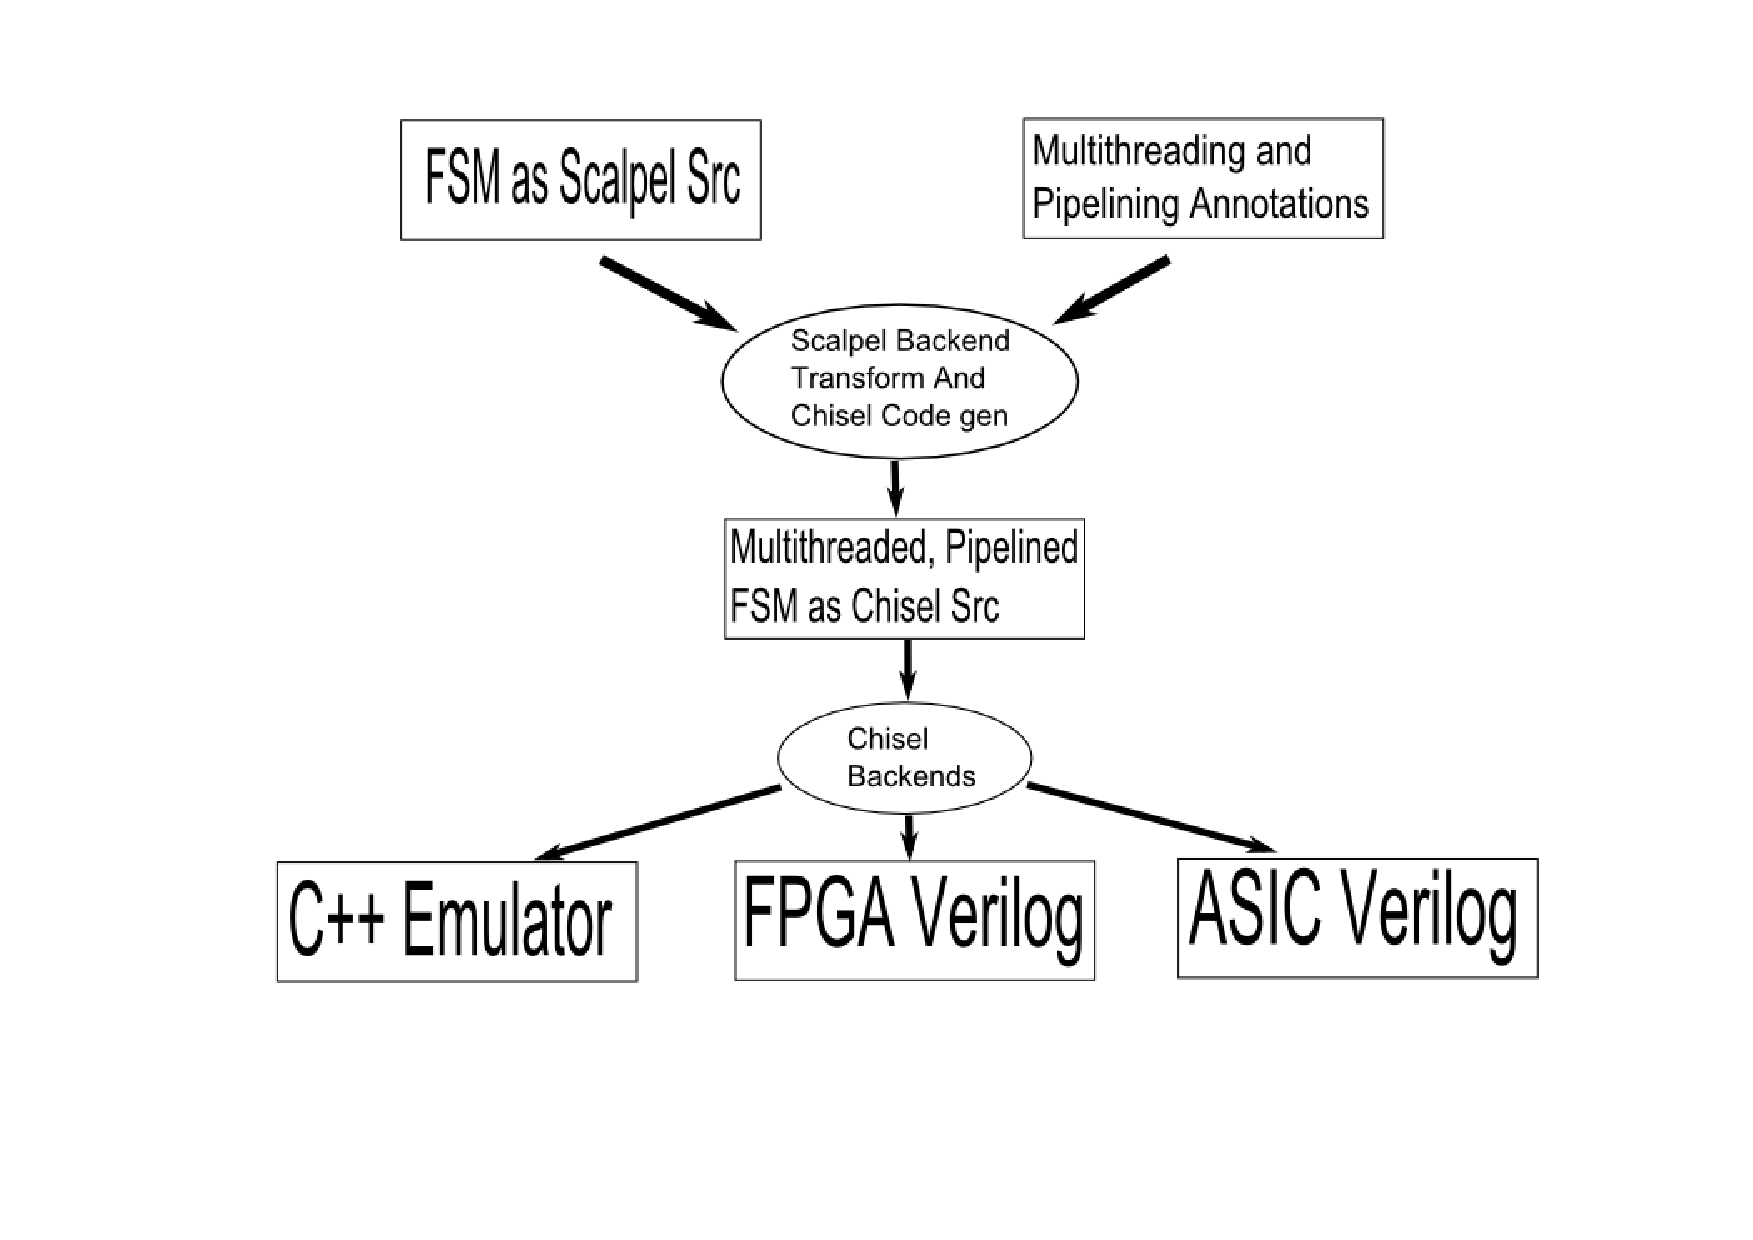
\includegraphics{figures/workflow}}
    \caption{Overall Tool Flow}
	\label{fig:workflow}
\end{figure*}

\section{Proposed Solution}
HLS produces designs with unacceptable performance, power, and area characteristics because the synthesis tool has to solve the computationally difficult problem of formulating a datapath that executes the dataflow graph and fits within the given performance, power, and area constraints. HLS tools do synthesize well optimized designs for specific patterns that occur in the high-level specification, so hardware designers working with HLS find themselves tuning high-level code to make specific synthesis tools produce exactly the datapath they want. 

This is clearly a case of automation trying to do too much. The HLS tools have a hard time formulating optimized datapaths, so the designers have to essentially tell the HLS tools what datapath they should use in a roundabout way by tuning the high-level specification. Clearly, designers would be more productive if they can specify the datapath directly. 

It seems like this conclusion tells us that designers should just do logic design using RTL in the traditional manner. However, much of traditional RTL specification deals with issues outside of simple datapath design. Logic designers spend much of their time specifying additional logic required to make the datapath fit performance, power, and area constraints. Some common optimization techniques include time-multiplexing functional units, pipelining, multi-threading, out-of-order execution, etc. These commonly used datapath optimization techniques can be captured as algorithms and applied automatically.

This thesis proposes a system in which the designer creates a RTL specification of the base functional datapath and separately specifies a series of optimizations to be performed on the datapath. Then automatic tools that know how to generically apply common optimization techniques can apply the specified optimizations to the base datapath and produce an optimized gate level specification to be fed into the next step in the IC design flow which may be physical design, fpga synthesis, or simulation. This system of specification will hence be referred to as Automatic Functional Datapath Optimization (AFDO). AFDO allows the designer to specify designers to specify a digital circuit with higher productivity than RTL specification without incurring the performance, power, and area penalties of HLS specification.

The automatic optimization tools discussed above work in the following manner. First, some initial processing transforms the RTL specification of the base datapath into a node graph data structure, where each node represents a digital circuit component(wire, combinational logic block, or state element) and each node contains input and consumer pointers to other nodes representing the topology of the circuit. Second, the tools implement the specified optimizations by modifying this node graph - creating new nodes, changing input/consumer pointers, copying existing nodes, etc. Third, the tool outputs the modified circuit in some specified representation

Although AFDO can be implemented if the base datapath is specified in discrete event simulation based RTL languages such as Verilog or VHDL, it is better for the base datapath should specified in a structural construction based RTL language such as Chisel. First, as mentioned in \ref{section:RTLCons}, discrete event simulator semantics are not particularly well suited for digital hardware specification and create a host of problems for the designer. Second, creating a node graph representation of the base datapath is much easier in structural construction based HDL languages such a Chisel as there is a one to one mapping between language construct and nodes in the node graph. In the case of Chisel, the automatic tools can directly operate on Chisel’s internal node graph data structure. In discrete event simulation based RTL languages, we have to first send the RTL specification through a gate level synthesis tool before we can construct the node graph data structure. This makes preserving names difficult and prevents the designer from using RTL level simulations of the automatically optimized designs. All of the automatic optimization tools discussed in the following sections apply transformations to base datapaths specified in Chisel or a reduced Chisel like RTL specifically designed to demonstrate AFDO.

AFDO increases logic designer productivity by addressing both limitations of RTL specification covered in \ref{section:RTLCons}. By usings a structural construction based RTL language like Chisel to specify the base functional datapath, the problems caused by discrete event simulator semantics are eliminated. By allowing the designer to specify only the base functional datapath, which is generally much less complex than the optimized design, and applying optimizations automatically, source code verbosity and algorithm obfuscation is eliminated. Now the designer can specify designs much faster and with fewer errors as he only has to specify the simple base functional datapata and use automatic tools to systematically apply the desired optimizations. Additionally, AFDO allows designers to more easily do design space exploration as they can produce new design points by simply selecting different optimization options for the automatic tools to apply instead of rewriting obfuscated RTL for each new design point. For example, adding a pipeline stage to a processor design in RTL is generally non-trivial in RTL because the pipeline control logic is entwined within the datapath specification. If the designer specifies a base functional 1 stage version of the processor and uses an automatic tool to pipeline the processor, adding a pipeline stage would be trivial on the part of the designer as he would simply have to tell the automatic pipeline tool to generate one more stage.

At the same time, AFDO retains performance, power, and area benefits of RTL specification by preserving a high level of correlation between language constructs and the generated hardware. The generated datapath is simply the base functional datapath modified with the designer specified optimizations. Unlike HLS, the designer knows the number and types of functional units used in the datapath as well as the state elements that are present in the datapath along with how those state elements are updated.

\section{Evaluation}

\section{AutoMArch}
AutoMArch is capable of creating multi-threaded in-order designs of any number of threads and any number of pipeline stages that is functionally equivalent to n-copies of the original base datapath, where n is the number of threads.

\subsection{Input Datapath Restrictions}
The input base functional datapath can be an arbitrary FSM with the following restrictions:

{\bf (1)} The input FSM must communicate to the outside world through ready/valid ports  

{\bf (2)} The designer cannot use input valid or output ready signals as inputs to any part of their circuit

{\bf (3)} Any functional units that may take more than one clock cycle to return responses(caches, multipliers, dividers, etc) must be accessed through the Variable Latency Unit Interface discussed below.

\subsubsection{IO Semantics}
When input ready or output valid is driven high by the input FSM, this implicity signals to the tool that the input FSM requires the use of the input or output port on the current state update. Thus, the tool generates logic that examines the input ready or output valid and stalls the pipeline if the corresponding input valid or output ready is not driven high by external modules. The designer should design the input FSM so that input readies and output valids are only driven high when absolutely necessary to avoid unnecessary stalling the automatically multi-threaded and pipelined version of the circuit.

\begin{figure}
	\centering
    \resizebox{\columnwidth}{!}{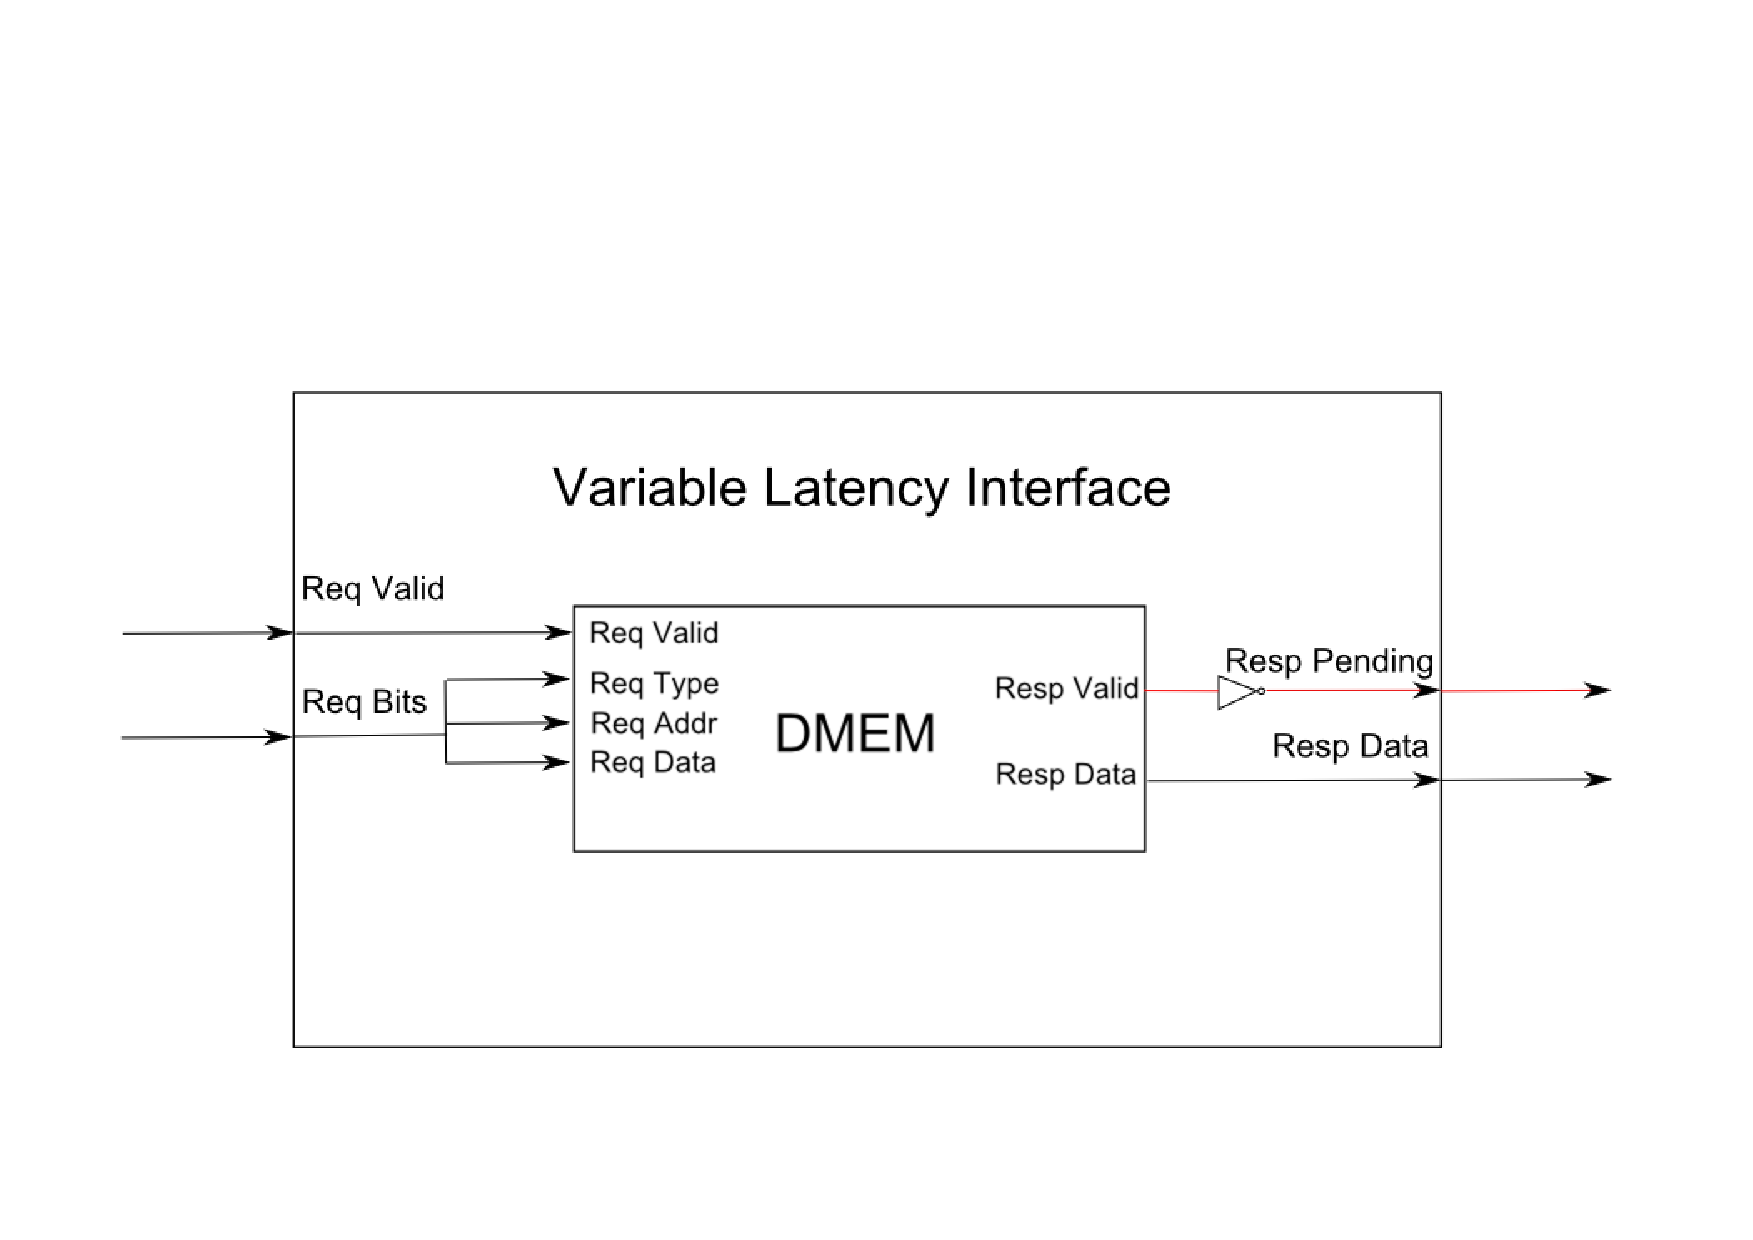
\includegraphics{figures/TransactionalInterface}}
    \caption{{\bf Single Thread View of Variable Latency Unit Interface} Black wire are user facing IO, red wires are tool facing IO}
	\label{fig:VarLatIO}
\end{figure}

\subsubsection{Variable Latency Unit Interface}
In order to accomodate caches and long latency arithmetic units in the minimal FSM specification that is not allowed to have any optimization or control logic implemented, the tool provides the Variable Latency Unit Interface. The designer should access any caches or long latency arithmetic units through a Variable Latency Unit Interface and treat that Variable Latency Unit Interface like a piece of combinational logic in the input FSM specification. IE the designer should not use the Resp Pending port of the Variable Latency Unit Interface to drive any part of their circuit and should pretend that the Variable Latency Unit Interface always gives a valid response immediately. The tool will automatically generate control logic that deals with the Variable Latency Unit Interface not immediately outputting a valid response.

\subsection{Automatic Pipelining}
\subsection{Automatic Multi-threading}

\section{AutoFAME}
\subsection{FAME Introduction}
FAME, or FPGA Architecture Model Execution is a system for efficiently emulating digital circuits on a FPGA introduced in the \textit{A Case for FAME: FPGA Architecture Model Execution paper} \cite{FAME:2010}. The paper introduces a system in which the concept of the emulated digital circuit, hence known as the target machine, is separated from the concept of the digital circuit that does the emulation of the target machine, hence known as the host machine. By extension, in FAME, the concept of time passing in the target machine, hence known as target time, is separated from the concept of time passing in the host machine, hence known as host time. 

In naive FPGA emulation, the target machine and the host machine are the same digital circuit. the RTL specification of the target machine is mapped directly to an FPGA through vendor tools with no change in the logic design. Because the characteristics of a FPGA are sometimes significantly different from the characteristics of a ASIC in timing and area characteristics, it is desirable to use a modified implementation of the design to emulation on a FPGA. In an modified implementation optimized for an FPGA, the host machine maybe different from the target machine and it may take more than one or less than one host clock cycle emulate one target clock cycle.

Using FAME, large digital designs can be broken up into modules that talk to each other in a decoupled manner. The partitioned system maintains the same target time behavior as the original design even though the modules are communicating in a decoupled manner. Once the original design is partitioned into decoupled modules, modules can be individually optimzed for FPGA emulation, with no restrictions on the host time to target time relationship in each module, while preserving the same target time behavior of the whole system as the target time behavior of the original design.

The original design to be emulated is called a FAME0 level design. The original design should be viewed as a set of FAME0 level modules connected together by registers and queues. A FAME0 module naively modified to work as a module that can be inserted into the partitioned system of decoupled modules is called a FAME1 level module. Figure \ref{fig:fame-partition} shows a FAME0 design being transformed intoa FAME1 design. A module that can be inserted into the partitioned system of decoupled modules and emulates a FAME0 module in an abstract manner, such as with a split functional model/timing model implementation of the FAME0 module, is called a FAME3 level module. A single module that can be inserted into the partitioned system of decoupled modules and emulates n copies of a FAME0 module through multi-threading is called a FAME5 level module. 

\begin{figure*}
	\centering
    \resizebox{1.5\columnwidth}{!}{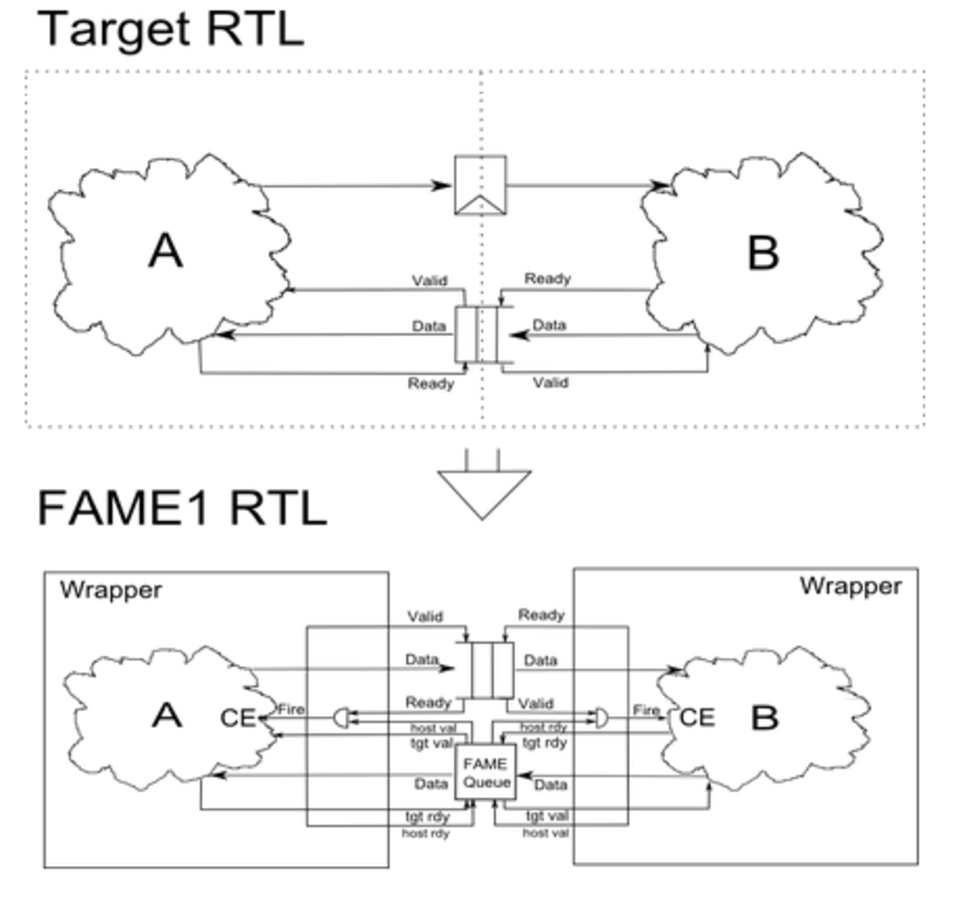
\includegraphics{figures/FAME-partition}}
    \caption{Transforming a FAME0 Design into a FAME1 Design}
	\label{fig:fame-partition}
\end{figure*}

\subsubsection{FAME Design Partitioning Details}
Target time behavior is maintained in the partitioned system in the following manner. The original design is partitioned by placing module boundaries across registers and queues in the target machine. The target machine registers are replaced by FAME Registers and the target machine queues are replaced by FAME Queues. The FAME Register is a FIFO containing tokens that represent the state of the target register at particular target clock cycles. Tokens furthur a ahead in the FIFO represent the state of the target register at earlier target clocks. The FAME Queue is a FIFO containing tokens that represent the state of the target queue at particular target clock cycles. Tokens furthur ahead in the FIFO represent the state of the target queue at earlier target clocks. Both FAME Registers and FAME Queues are initialized with one token. 

It is important to separate these tokens, which represent one target clock cycle's worth of information about the target register or target queue, from the entries in the target queues. Enqueuing/dequeuing tokens from FAME Registers/FAME Queues will be referred to as host enqueue/host dequeue and the host enqueue/dequeue operations will be performed through manipulating host ready and host valid signals. If a FAME Register/FAME Queue does not contain any tokens, it will be referred to as host empty and if a FAME Register/FAME Queue cannot accept any more tokens, it will be referred as host full. In contrast, enqueueing/dequeue entries from the target queues will be referred to as target enqueue/target dequeue and the full/empty status of the target queues will be referred to as target full/target empty.

For every advance of the target clock, each module consumes a token from its input FAME Registers/FAME Queues and outputs a token to its output FAME Registers/FAME Queues. A module may not advance its target clock if any of its inputs are host empty or if any of its outputs are host full. Since FAME Registers and FAME Queues are FIFOs of tokens, tokens are allowed to accumulate with in FAME Registers and FAME Queus. Thus, the target clock can advance in a decoupled manner while still remaining functionally the same as the original design. 

\subsubsection{AutoFAME Features}
AutoFAME is capable of creating FAME1 and FAME5 level FPGA optimized designs given a base functional datapath specified in Chisel. This is equivalent of automatically transforming a FAME0 level design into a FAME1 or FAME5 level design. The tool performs the required circuit transformations on the Chisel internal node graph and leverages Chisel's elaboration steps to output the optimzed design as either a cycle accurate C++ emulator or as a Verilog source file. 

\subsection{Input Datapath Restrictions}
\label{section:fameRestrictions}
Because the orignal design to be emulated should be split by having module boundaries placed across registers or queues, the input FAME0 module should have IO ports of the type RegIO, which consists of a single data pin and indicates that the IO port should be connected to a register in the original design, and QueueIO, which consists of a ready pin, a valid pin, and a data pin, and indicates that the IO port should be connected to a queue in the original design.

\subsection{FAME1 Transform}
Given any FAME0 module that follows the restrictions in \ref{section:fameRestrictions} and a user annotation in the Chisel source file containing the module instantiation of the input FAME0 module that a FAME0 to FAME1 transformation should be applied, AutoFAME will produce a FAME1 version of that module.

Automatically transforming a FAME0 level design into a FAME1 level design is useful because it allows the FAME0 level design to be interfaced with FAME3 or FAME5 level designs at the cost of no extra work by the designer.

\subsubsection{Transformation}
In order to make a FAME0 module work in the partitioned system of decoupled modules, its RegIOs need to be converted into FAMERegIOs, which attach a host ready and a host valid pin to the RegIO port in order to interface with the FAME Registers. Its DecoupledIOs also need to be converted into FAMEDecoupledIOs, which also attach a host ready and a host valid pin to the DecoupledIO in order to do host enqueue/dequeues.

Then every state element write enable signal is masked with a fire target clock signal. The fire target clock signal is driven low whenever any of the input FAME Registers/FAME Queues are host empty or any of the output FAME Registers/FAME Queues are host full.

Then combinational logic is generated to host dequeue the input FAME Registers/FAME Queues and enqueue the output FAME Registers/FAME Queues whenever fire target clock is high.

\subsubsection{Example Application}
Automatic FAME0 to FAME1 transformation was used to interface a FAME0 level high performance research RISC processor used by UC Berkeley's ASPIRE Lab with a FAME3 level hardware DRAM model for FPGA emulation. The hardware FAME3 level DRAM model is necessary to get accurate results for the processor in FPGA emulation because the relative DRAM to processor clock rate on a FPGA is much higher than the relative DRAM to processor clock rate on a ASIC. In order to obtain performance figures accurate to the ASIC implementation in emulation, the FAME3 hardware DRAM model is used as a intermediary between the processor and the FPGA DRAM and makes the FPGA DRAM appear slower to the processor. Additionally, the FAME3 hardware DRAM model can be adjusted to simulate a variety of DRAM configurations, which would not be possible if the processor interfaced directly with the FPGA DRAM.

\subsection{FAME5 Transform}
Given any FAME0 module that follows the restrictions in \ref{section:fameRestrictions} and a user annotation in the Chisel source file containing the module instantiation of the input FAME0 module that a FAME0 to FAME5 transformation should be applied along with a specification of how many threads there should be, AutoFAME will produce a FAME5 version of that module.

Automatically transforming a FAME0 module into a FAME5 level design is useful because it allows the designer to conserve area usage on the FPGA if the FAME0 level design is instantiated many times as the multi-threading only replicates the state elements and not the combinational logic in the FAME0 design. Additionally, the multi-threading allows external memory access latencies to be hidden.

\subsubsection{Transformation}
First, all of the IO ports and the state elements are replicated n times, where n is the user specified number of threads.

Then, like the FAME0 to FAME1 transformation, the RegIOs and Decoupled IOs the input FAME0 design are replaced with FAMERegIOs and FAMEDecoupledIOs.

Then, a IO Ready signal and a Thread Selected signal is generated by each thread. The IO Ready signal of thread m is driven high when all of the input ports associated with thread m are not host empty and all of the output ports associated with thread m are not host full. The Thread Selected signal for thread m is high when the thread select id generated by the thread scheduler equals m.

Then, a fire target clock signal is created for each thread. Thread m's fire target clock signal when thread m's IO Ready signal is high and thread m's Thread Selected Signal is high. The write enables of all the state elements associated with thread m are then masked with the fire target clock signal of thread m.



\section{Conclusion and Future Work}
In this thesis, I presented a system for digital circuit frontend specification named Automatic Functional Datapath Optimization. In this system, the designer specifies a base functionally correct datapath without any optimizations applied in a RTL like manner and then selects optimization techniques for automatic tools to apply to the base functional datapath. This system of specification is a middle ground approach between RTL specification and HLS specification and tries to capture the conflicting pros of both approaches, namely high designer productivity and the ability to generate highly efficient designs in terms of performance, power, and area at the same time. I implemented two examples of such a system, AutoMArch and AutoFAME, and presented example applications of both.

I hope that AutoMArch can be extended to support more general speculation and that a more general form multi-threading, where combinational logic is replicated as well as the state elements can be explored. I also hope that work can be done to catalogue all of the commonly used digital circuit optimization techniques so that they may one day be implemented automatically

\clearpage
\bibliographystyle{abbrvnat}
\setlength{\bibsep}{0.0pt}
\renewcommand*{\bibfont}{\footnotesize}
\bibliography{references}

\end{document}
